\documentclass{tpu-sotu}
\usepackage{ascmac}
\usepackage{cite}
\usepackage[dvipdfmx]{hyperref,graphicx}
\usepackage{pxjahyper}
\usepackage{listings}
\lstset{
basicstyle={\small},% 
identifierstyle={\small},% 
commentstyle={\small\ttfamily \color[rgb]{0,0,0}},% 
keywordstyle={\small\bfseries \color[rgb]{0,0,1}},% 
ndkeywordstyle={\small},% 
stringstyle={\small\ttfamily}, 
frame={tb}, 
breaklines=true, 
columns=[l]{fullflexible},% 
xrightmargin=0zw,% 
xleftmargin=3zw,% 
numberstyle={\scriptsize},% 
stepnumber=1, 
numbersep=1zw,% 
morecomment=[l]{//}% 
}
%
% ここでタイトルの設定をします
%
% 自分の名前
\author{尾崎 裕樹}
%
% 学籍番号
\gakusekibangou{1515015}
%
% タイトル
\title{プログラミング演習における模範解答を用いた\\テストケース評価基準の自動生成}
\etitle{English Title}
%
% 日付
\date{2018年2月}
%
% 指導教員
\professor{中村 正樹 准教授}
%
% 所属
\department{電子・情報工学科}
%
%----- begin document
%
\begin{document}
%
\maketitle
\clearpage
\pagenumbering{roman}
\tableofcontents
\clearpage
\pagenumbering{arabic}
%

% - - - - - - - - - - - - - - - - - - -
%
\chapter{はじめに}
本研究では、プログラミング教育において、教員が学生の作成したプログラムに対して適切な評価を行う方法を考え、その際に利用できるシステムを提案する。
\section{背景}
プログラミング演習おいて、学生は最初に教科書のソースコードを書き写すことから始める。教科書のコードが正確に書き写せているかの確認をするには、教員が正しいソースコードを用意し学生の書き写したソースコードと比較すればよい。しかし、ただ教科書のソースコードを書き写すだけではプログラムを作成できるようにはならないので、プログラミング演習では提示された仕様を満たすプログラムを作成することを学ぶ必要がある。仕様を見てプログラムを作成した場合に教員と学生が同じ実装をするとは限らないため、教員のソースコードと学生のソースコードを単純に比較しただけでは正確な評価はできない。そこで、テストケースを設計してプログラムのテストを行うことによって学生が作成したプログラムを評価する。このテストケースを学生自身が適切に設計できるようになるためには、設計したテストケースを評価できなければならない。しかし、テストケースは境界値以外の値は答えが単一ではない。したがって、学生が設計したテストケースと教員が設計したテストケースが合致しなかったとしても、学生のテストケースが誤りであるとは限らない。つまり、テストケースを評価する場合も、教員のテストケースと学生のテストケースを単純に比較しただけでは正確な評価ができないため、テストケースの評価方法を考える必要がある。

例えば文献~\cite{a0}では、テスト駆動開発に基づきプログラミング演習を行うことによってコーディングだけでなく、ソフトウェアテストの学習が行われる。評価対象は学生のプログラムとテストケースで、教員の作成したプログラムとテストケースを用いて図1.1のようにトリプルチェックを行うことによって評価される。
\newpage
\begin{figure}[h]
  \centering
  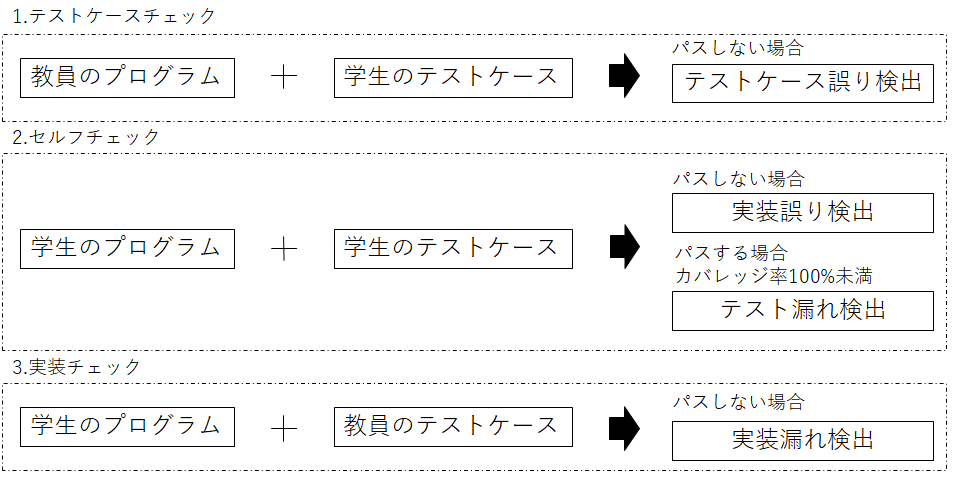
\includegraphics[width=130mm]{トリプルチェック.png}
  \caption{トリプルチェックによるコード判定原理}
\end{figure}

テストケースチェックによって、仕様要求を満たしていないテストケースが検出され、学生のテストケースの間違いが早期に指摘される。なお、仕様要求とは、プログラムにおける関数あるいはサブルーチンの動作が規定されたものであり、戻り値や引数などが定められたものである。教員のプログラムとテストケースはこの仕様要求が満たされるとする。
次のセルフチェックでは、テストの実行だけでなくコードカバレッジの測定が行われる。テストにパスしない場合は、学生のプログラムが正しく実装されていないことが分かり、テストにパスしたが、カバレッジが100\%でない場合は、テスト漏れが検出され学生に指摘される。最後の実装チェックでは、学生のプログラムが仕様要求の要求をすべて満たしていないことが検知され、次のテスト駆動開発サイクルを始めるよう学生に通知される。実装チェックをパスすることによって、学生が作成したプログラムとテストケースが仕様要求の要求をすべて満たしたことが確認される。

しかし、この手法では学生が仕様通りのプログラムを作成した後に仕様通りのテストケースであるかの確認が行われるため、学生が自身のテストケースを用いてプログラムの確認を行うことはできない。
\section{目的}
本研究では、学生がテストケースを設計できる
\section{論文の構成}
  ・・・
\chapter{プログラミング演習におけるテストケース評価システム}
本章では文献~\cite{a1}で提案されているテストケース評価システムについて紹介する。テストケース評価システムでは、学生自身が適切なテストケースを設計できるようになるために、学生が作成したテストケースを評価してアドバイスを行うシステムが提案されている。このシステムでは、教員が演習問題毎にテストケースの評価基準とテストケースが不足していた場合に表示するアドバイスを与える必要がある。演習問題毎にテストしなければならない値や入力のデータ数が異なるため、評価基準は演習問題を分析した上で、入力のデータ構造を定義してから記述される。
\section{テストケース評価システム}
テストケース評価システムでは、教員があらかじめテストケース評価基準を作成し、学生が設計したテストケースが評価基準をどの程度パスできるかを判定することによって、テストケースの評価が行われる。評価基準をパスしない場合にアドバイスを表示することで、不足しているテストケースを学生に知らせる。テストケース評価システムにおいて、評価基準は次のようにタブ区切り形式でテキストとして記述される。

\begin{minipage}[b]{.7\textwidth}
\begin{itembox}[l]{評価基準の記述形式}
{\tt
 評価基準番号 TAB 判定条件 TAB アドバイス
}
\end{itembox}
\end{minipage}

「判定条件」はテストケースにおける入力データが満たすべき条件で、その条件を満たすテストケースがなかったときに、学習者に「アドバイス」が表示される。同値クラスを評価するための基準が複数ある場合などは、同じ「評価基準番号」を指定することで、評価基準がグループ化できる。例えば、年齢(整数値)を入力して、20歳以上は成年、20歳未満は未成年と表示する課題の評価基準は、入力データを変数ageとして、成年、未成年、エラーの場合について次のように記述される。

\begin{minipage}[b]{.7\textwidth}
\begin{itembox}[l]{評価基準の記述例1}
{\tt
1 TAB age==20 TAB 成年の最低年齢

1 TAB age>=20 TAB 成年の場合

2 TAB age==19 TAB 未成年の最高年齢

2 TAB age==0 TAB 0歳

2 TAB age>=0 \&\& age<20 TAB 未成年の場合

3 TAB age<0 TAB 年齢がマイナスの場合
}
\end{itembox}
\end{minipage}

学生が作成したテストケースの網羅率を、次の式で定義される評価基準のテストカバレッジにより提示する。

\begin{minipage}[b]{.7\textwidth}
\begin{itembox}[l]{評価基準のテストカバレッジ(%)}
{\tt
学習者のテストケースがパスした評価基準グループ数÷\\教員が記述した評価基準グループ数×100
}
\end{itembox}
\end{minipage}

判定条件の記述において、課題毎に入力データの型や個数が異なるため、テストケースの入力のデータ構造を定義し、そこで定義された変数を用いて判定条件が記述される。
\section{入力のデータ構造の定義}
データ構造は型と変数と出現回数から成る。入力のデータ構造の記述法はバッカス・ナウア記法(BNF)に類した形式で設計された。入力のデータ構造の定義例を以下に示す。なお、* は0回以上の繰り返しを表し、pintは正の整数、uintは0と正の整数、udoubleは0と正の実数の型である。

\begin{minipage}[b]{1.025\textwidth}
\begin{itembox}[l]{データ構造の定義例}
(A)データ数(n)を入力し、その個数分身体データを入力する場合
{\tt

(pint n)

(pint id, string name, uint age, udouble height, udouble weight)\{n\}
}

(B)ファイルの終端まで分身体データを入力する場合
{\tt

(pint id, string name, uint age, udouble height, udouble weight)\{*\}
}

\end{itembox}
\end{minipage}

\section{関数定義}
判定条件の記述に関数を用いることができる。複数の身体データを読み込んで、身長の最大値を表示する課題の場合、最大値が複数存在するテストの評価基準は、引数のリストの最大値の個数を返す関数countmax()を定義して、次のように記述される。なお、実引数heightは全身長データのリストである。関数を評価基準で用いる場合、教員は関数定義も与える必要がある。

\begin{minipage}[b]{.8\textwidth}
\begin{itembox}[l]{関数を用いた評価基準の記述例}
{\tt
1 TAB countmax(height)>=2 TAB 身長の最大値が複数の場合
}
\end{itembox}
\end{minipage}
\begin{lstlisting}[caption = countmax 関数, basicstyle=\ttfamily\footnotesize, frame=single]
function countmax($list){

	$lmax = max($list);

	return count(array_keys($list, $lmax));

}
\end{lstlisting}

\section{評価基準の具体例}
入力が比較的複雑になる課題として、ボウリングの得点計算が例示されている。
\begin{itembox}[l]{ボウリングの点の計算の課題}
ボウリングは、1フレーム目から10フレーム目までの倒れたピンの数によって得点が決まる。フレームごとに倒したピンの数を読み込み、各フレームごとの得点を計算して表示すること。なお、ガーターとミスは0と表示するものとし、ダブルがあった場合はメッセージを表示する。
\end{itembox}
\begin{minipage}[b]{.7\textwidth}
\begin{itembox}[l]{ボウリングのデータ構造}
{\tt
(uint thr1, uint thr2)\{9\}

(uint last1, uint last2, uint last3)
}
\end{itembox}
\end{minipage}
\begin{itembox}[l]{ボウリングの評価基準}
{\tt
1 TAB thr1 == 10 TAB ストライクのスコア計算

2 TAB thr1 != 10 \&\& thr1+thr2 == 10 TAB スペアのスコア計算

3 TAB last1 == 10 TAB ストライクの通常加算

3 TAB last1 != 10  \&\& last1+last2 == 10 TAB スペアの通常加算

4 TAB double\_strike(thr1) || all\_strike([last1, last2]) TAB ダブル

4 TAB last\_strike(thr1) == 1 \&\& last1 == 10 TAB 最終Fをまたぐダブル
}
\end{itembox}

ストライクとスペアだった場合のスコア計算が正しいかをテストする必要がある(評価基準番号1, 2)。最終フレームではストライク、スペアでも通常の加算になるので、それらのテストも必要である(評価基準番号3)。評価基準番号4はダブルについてのテストである。ダブルがあればtrueを返す関数double\_strike()、 リストがすべて10ならばtrueを返す関数all\_strike()、リストの最後の要素から10が何回連続しているかを返す関数last\_strike()が定義されている。
\section{システムの評価}
参考書の例題のテストケースのデータ構造が評価システムに則した形式で記述できるか調査が行われ、実行時に入力のデータ構造が変化する共用体などの問題以外ではデータ構造を記述できることが確認された。

また、評価システムにより、学生がテストケースを作成できるようになるのか確認をするために、プログラミングを学習済みの学生7人が評価システムを使ってボウリングの課題のテストケースを作成した。その結果最終的に6人の学生がカバレッジ100\%を達成したことが確認された。
\section{システムの課題}
テストケース評価システムでは、教員が問題文を分析した上で、評価基準を記述しているので、システムを運用する上で教員の負担が大きくなってしまうことが考えられる。そこで、本研究は教員の負担を減らすために、評価基準を自動で生成する方法を提案する。
\chapter{テストケース評価基準の自動生成}
\section{背景}
\chapter{検証}
\section{背景}
\chapter{おわりに}
\acknowledgements
\begin{thebibliography}{2}
   \bibitem{a0} 吉田英輔,角川裕次: テスト駆動開発に基づくプログラミング学習支援システム : 初心者開発者のためのセルフトレーニングアーキテクチャ,信学技報.\\SS,ソフトウェアサイエンス,Vol.105,No.331(2005),pp.27-32
   \bibitem{a1} 蜂巣吉成,小林悟,吉田敦,阿草清磁: プログラミング演習におけるテストケース評価システム,コンピュータソフトウェア第34巻第4号,2017,pp.54-60
\end{thebibliography}

\end{document}
